\newlength{\bibsep}
\documentclass[nonatbib,5p,a4paper]{elsarticle}  % 5p for two columns, 1p for 1 column (this is specific for the elsearticle)
\usepackage[english,norsk,nynorsk]{babel}        % Language
\usepackage[DatePublished]{Code/NTNU-lab}        % remove [DatePublished] to remove dates
\usepackage{csquotes}                            % Must be loaded when babel is loaded to avoid error.
% Use this file to write code that you do not want in the .sty file, but has to be in the preamble (before \begin{document}).
% Writing in this file in stead of in the preamble will keep the main file more organised and tidy.


%                       Nomenclatures
%_______________________________________________________________
\usepackage[intoc]{nomencl}
\makenomenclature

\renewcommand{\nomname}{%
% Title
%----------------
List of Symbols
%----------------
}
\renewcommand{\nompreamble}{%
% Description
%----------------
The next list describes several symbols that will be later used within the body of the document
%----------------
}
% This code creates the groups
\renewcommand\nomgroup[1]{%
  \item[\bfseries
  \ifstrequal{#1}{A}{Physics constants}{%
  \ifstrequal{#1}{B}{Mathematical constants}{%
  \ifstrequal{#1}{C}{Other symbols}{}}}%
]}
% This will add the units
\newcommand{\nomunit}[1]{%
\renewcommand{\nomentryend}{\\#1}}
%................................................................

                            % Write all preamble code in this file to keep it organised and tidy.

\addbibresource{Bibliography/Sources.bib}        % Selects the Bibliography file.


\begin{document}
\selectlanguage{english}                         % Sets the language of the document.

%%%%%%%%%%%%%%%%%%%%%%%%%%%%%%%%%%%%%%%%

\begin{frontmatter}
%
% Title:
%------------------------------------
\title{%
Stable Coin Return Analysis\\
\small Relating Volatility to the Obtainable Return on Stable Coins  % A good idea is to have the subject code and name as subtitle
}
%
% Authors:
%------------------------------------
% List an author with name ' Firstname Middlename Lastname ' like this:
% F. M. Lastname
\author[address]{J. H. Gruenewald} 
\address[address]{https://github.com/johngru}
%
% Date:
%------------------------------------
%
\newdate{dateName}{23}{05}{2022} % edit the date here, ' dateName ' has to match on these two lines.
\renewcommand*{\today}{\DayMonthYearDateFormat\displaydate{dateName}} 
% Options for displaying date: \MonthYearDateFormat,  \DayMonthYearDateFormat or \YearDateFormat
%
% Abstract:
%------------------------------------
\NameOfAbstract{Abstract} % Change abstract title here. 
\begin{abstract}
% Delete the text and write your abstract here:
%------------------------------------

In volatile crypto markets, the price of a stable coin often fluctuates around its intended \textit{pegged} value.  This analysis relates the stable coin's volatility to the maximum potential return achieved by trading on the stable coin's price swings.  Unlike other asset classes, the achievable return on stable coins, or any asset tied to a constant value, is found to be directly proportional to the sum of its price variance and covariance.  

\end{abstract}
%
\end{frontmatter}
%
%
% Table of contents:
%------------------------------------
% If the report is very long for some reason (over 4 or 5 pages), use a table of contents.
% Uncomment everything below the line ---- to get table of contents (ctrl + /) (the / on numberpad):
%-------------
%
% \ 
% \vspace{1cm}

% \begin{minipage}{\textwidth}
%     \tableofcontents
% \end{minipage}
% \clearpage
%% Prints a list of symbols. You can create/ change the categories in the preamble.tex file. 
% Learn more about nomenclature: https://www.overleaf.com/learn/latex/Nomenclatures
%
% Delete/change the text and write your Nomenclature here:
%------------------------------------

\nomenclature[A, 02]{\(c\)}{\href{https://physics.nist.gov/cgi-bin/cuu/Value?c}
{Speed of light in a vacuum}
\nomunit{\SI{299792458}{\meter\per\second}}}
\nomenclature[A, 03]{\(h\)}{\href{https://physics.nist.gov/cgi-bin/cuu/Value?h}
{Planck constant}
\nomunit{\SI[group-digits=false]{6.62607015e-34}{\joule\per\hertz}}}
\nomenclature[A, 01]{\(G\)}{\href{https://physics.nist.gov/cgi-bin/cuu/Value?bg}
{Gravitational constant} 
\nomunit{\SI[group-digits=false]{6.67430e-11}{\meter\cubed\per\kilogram\per\second\squared}}}
\nomenclature[B, 03]{\(\mathbb{R}\)}{Real numbers}
\nomenclature[B, 02]{\(\pi\)}{Pi}
\nomenclature[B, 01]{\(e\)}{Euler's constant}
\nomenclature[C]{\(V\)}{Constant volume}
\nomenclature[C]{\(\rho\)}{Friction index}

% Print statement:
%--------------------
\printnomenclature                 % List of symbols, can be useful
\section{Analysis}
% Delete the text and write your Introduction here:
%------------------------------------


%\begin{figure}
%    \centering
%    
\includegraphics[width=0.48\textwidth]{Images/PNG-example.png}
%    \caption{Example image in png format, taken by yours truly.}
%    \label{fig:NTNU-letters}
%\end{figure}

For a general stable coin, its price is pegged to a constant value $c$.  That is, there are active market forces maintaining the price at its pegged price and the price of the coin will predominantly hold this value.  If its price is actively being maintained at $c$, then the average value ${\mu}$ of a stable coin's price will be equal to its pegged value.   That is, we assume:
\begin{equation}
    \mu = c
\end{equation}
For any time the price deviates from its peg, it can be traded and the total return $R_{TOT}$ is:
\begin{equation}
    R_{TOT} = \sum\limits_{j}{(P_{j} - \mu)/\mu},
\end{equation}
where $P_{j}$ is the current stable coin price off the peg value.  For simplicity, let's define the difference between the stable coin's price and peg value as $Z_{j}$ or $Z_{j} = (P_{j}-\mu)$.
To find a relationship between $R_{TOT}$ and the volatility, we can make the following mathematical substitutions:
\begin{equation}
    R_{TOT}^2 = \frac{1}{\mu^2}[\sum_j{Z_j}]
\end{equation}
And letting $\mu^2 = 1$:
\begin{equation}
    R_{TOT}^2 = \sum_j{Z_j^2} + \sum\limits_{j\neq i}{Z_j Z_i}
\end{equation}
Now substituting in for $Z_j , Z_i$ and multiplying by an identity:

\begin{equation}
   R_{TOT}^2 = \sum_j{(P_{j}-\mu)^2} + \sum\limits_{j\neq i}{(P_{j}-\mu) (P_{i}-\mu)} \notag
\end{equation}
\begin{equation}
        = \frac{N-1}{N-1} \times [\sum\limits_{j}{(P_{j}-\mu)^2} + \sum\limits_{j\neq i}{(P_{j}-\mu) (P_{i}-\mu)}] \notag
\end{equation}
\begin{equation}
    = (N-1) \times [\sigma^2(P_j) + Cov_{i \neq j}(P_i,P_j)] 
\end{equation}
or taking the root of both sides relates the total return to the variance and covariance:
\begin{equation}
  \boxed{R_{TOT}=\sqrt{(N-1) \times [\sigma^2(P_j) + Cov_{i \neq j}(P_i,P_j)]}}
\end{equation}



%\subsection{Problem Description}
%Consider using dividing the introduction and other sections of the report into different parts using %\verb+\subsection+. This will make the report more reader friendly. 


%% Place large figures that span the whole width of the page in here to easily move them around in the file
% and to avoid getting figures displayed after references and appendix. 
%
% Use {figure*} for a figure that will span both columns. 
% Below is an example of a figure with 6 sub-figures.
\begin{figure*}
%
        \subfigure[Contour plot number 1]{%
            \label{fig:Contour_1}
            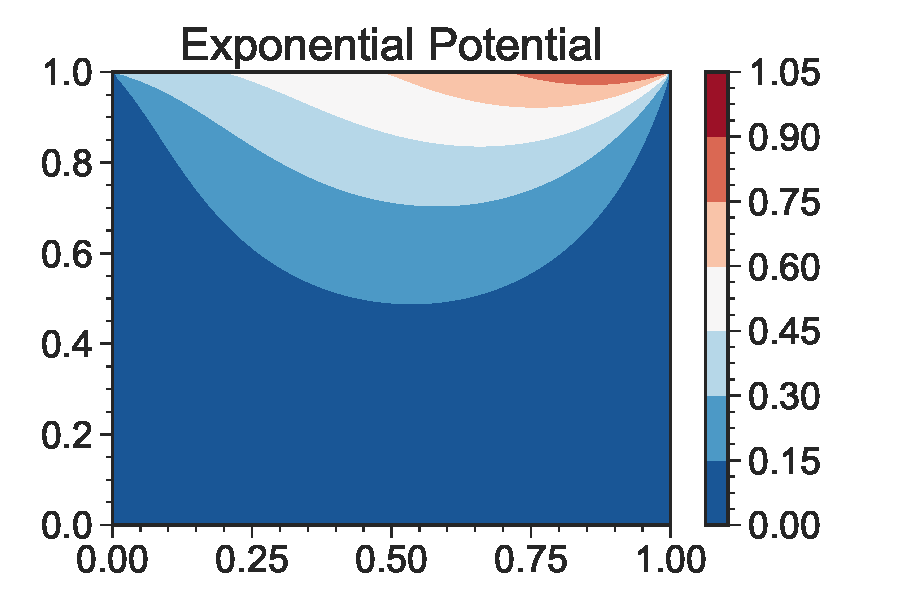
\includegraphics[width=0.3\textwidth]{Images/Fig:Countour-plot/1-contour.pdf}
        }%
        \hspace{1em}
        \subfigure[Contour plot number 2]{%
            \label{fig:Contour_2}
            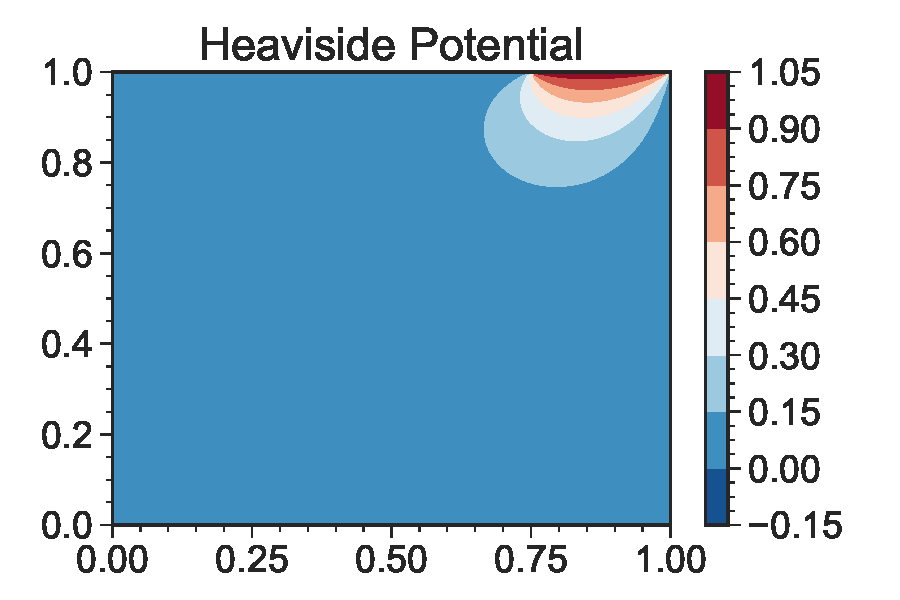
\includegraphics[width=0.3\textwidth]{Images/Fig:Countour-plot/2-contour.pdf}
        }%
        \hspace{1em}
        \subfigure[Contour plot number 3]{%
           \label{fig:Contour_3}
           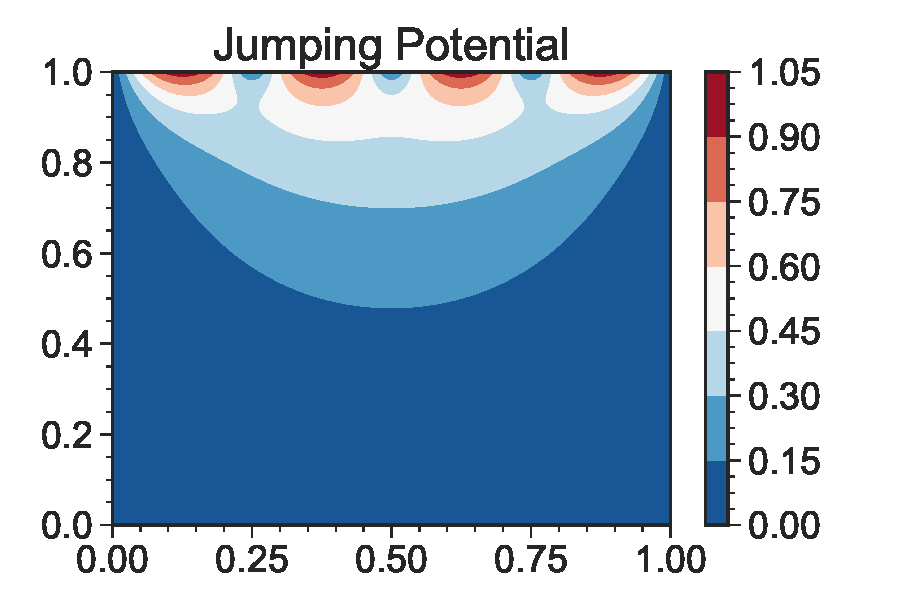
\includegraphics[width=0.3\textwidth]{Images/Fig:Countour-plot/3-contour.pdf}
        }\\ %  ------- End of the first row ----------------------%
        \subfigure[Contour plot number 4]{%
            \label{fig:Contour_4}
            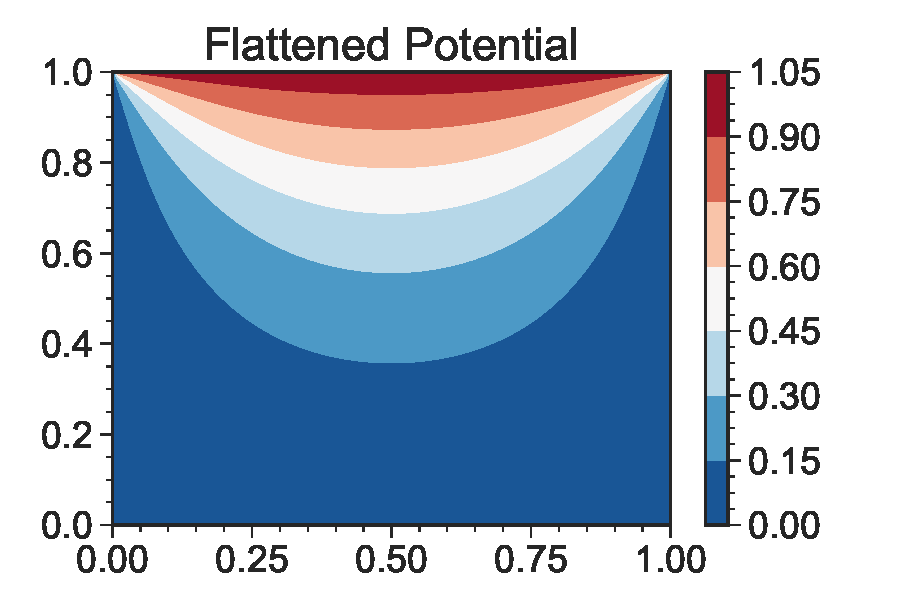
\includegraphics[width=0.3\textwidth]{Images/Fig:Countour-plot/4-contour.pdf}
        }%
        \hspace{1em}
        \subfigure[Contour plot number 5]{%
            \label{fig:Contour_5}
            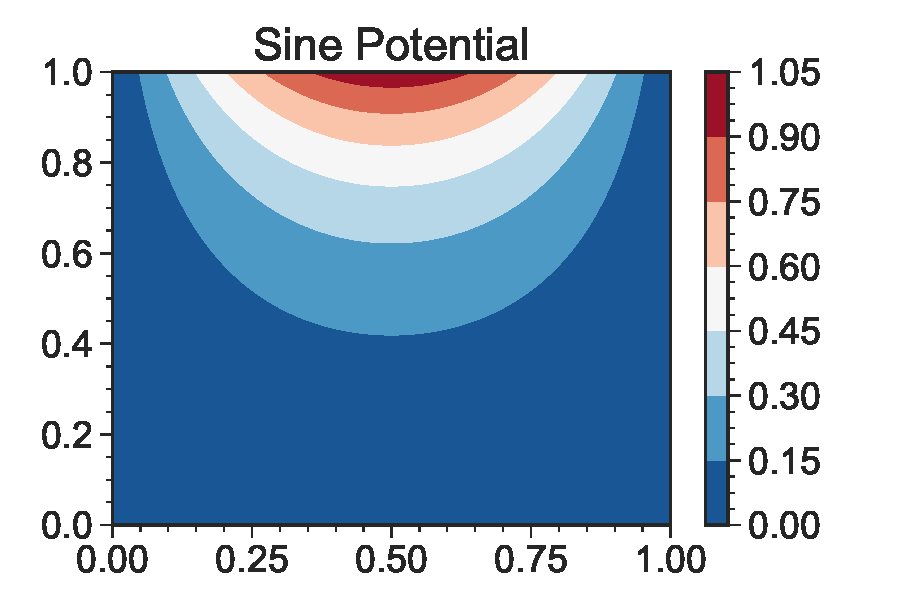
\includegraphics[width=0.3\textwidth]{Images/Fig:Countour-plot/5-contour.pdf}
        }%
        \hspace{1em}
        \subfigure[Contour plot number 6]{%
            \label{fig:Contour_6}
            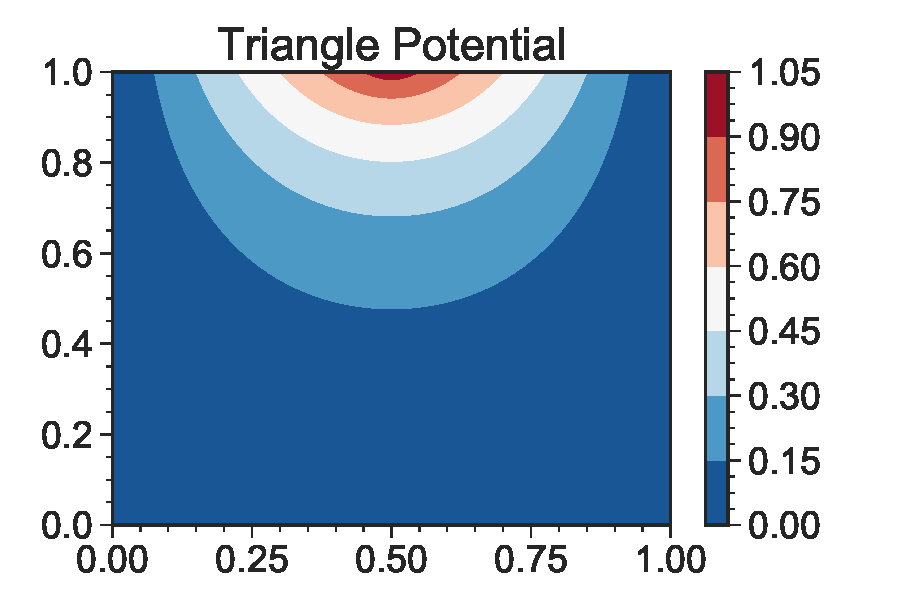
\includegraphics[width=0.3\textwidth]{Images/Fig:Countour-plot/6-contour.pdf}
        }%
%
    \caption{%
        Contour plots for different potentials $V_0(x)$, along the line $y=1$
     }%
   \label{fig:Countour-plot}
\end{figure*}                     % Change this to another line to move big figures.
\section{Skeleton Code}
\definecolor{light-gray}{gray}{0.95}
\newcommand{\code}[1]{\colorbox{light-gray}{\texttt{#1}}}
% Delete the text and write your Theory/ Background Information here:
%------------------------------------

A code outline for running a trading bot on stable coins. \par
\textbf{Skeleton Code:}
\newline
\code{def run(NOT STOP):}\\
\code{\indent \indent peg = 1}\\
\code{\indent \indent currency = "USD"} \\
\code{\indent  \indent stable\_coin = "USDC"} \\
\code{\indent \indent action = \{ 'BUY','SELL','HOLD' \} } \\
\code{\indent \indent fees} \\
\code{\indent \indent cost\_avg} \\
\code{\indent \indent conditions = \{\}} \\
\code{\indent \indent search = TRUE} \\
\code{\indent \indent stop = FALSE} \\
\code{\indent \indent current\_price = get\_price(stable\_coin)} \\
\newline
\code{\indent while(search):} \\
\code{\indent \indent \indent previous\_price = current\_price} \\
\code{\indent \indent \indent current\_price = get\_price(stable\_coin)} \\
\code{\indent \indent \indent difference = price\_compare(current\_price,}
\code{\indent \indent \indent \indent previous\_price)} \\
\code{\indent \indent \indent action\_needed = action\_needed(difference,} \\
\code{\indent \indent \indent \indent conditions)} \\ 
\code{\indent \indent \indent if(action\_needed):} \\
\code{\indent \indent \indent \indent search = FALSE} \\
\code{\indent \indent \indent rest()}
\newline
\code{\indent \indent if(action\_needed == 'BUY'):} \\
\code{\indent \indent \indent API\_request(buy\_action)} \\
\code{\indent \indent \indent update(portfolio, cost\_avg)} \\
\code{\indent \indent \indent search = TRUE}
\newline
\code{\indent \indent if(action\_needed == 'SELL'):} \\
\code{\indent \indent \indent API\_request(sell\_action)} \\
\code{\indent \indent \indent update(portfolio, cost\_avg)} \\
\code{\indent \indent \indent search = TRUE}
\newline
\code{\indent \indent if(action\_needed == 'STOP'):} \\
\code{\indent \indent \indent stop = TRUE}

%\code{\indent  while(search):} \\
%\code{\indent \indent  current_price = get_price(stable_coin)} \\


%\section{Method and Equipment}
% Delete the text and write your Method(s) here:
%------------------------------------

An important quality of a scientific report is that it should be possible to redo the experiment based on the
information found in the report.
However, this does not mean that you should write every detail. Only include parts necessary to obtain the final result.
Specific details like serial numbers, manufacturer, etc. goes in your lab journal, an appendix, or can be mentioned briefly if it is relevant to the discussion. Remember that a scientific report should be short. \par
Remember to use helpful figures and refer to them. In \cref{fig:Countour-plot} you can see examples of vector graphics images. \par
You can also mention \textit{noteworthy} safety measures you took during the experiment in this section of the report.

%\section{Results}
% Delete the text and write your Results here:
%------------------------------------

The results section can be combined with the discussion if appropriate. In case of many sub\-/experiments % \-/ fixes the problem that LaTeX won't hyphenate words with dashes in them.
where the results are vaguely related or unrelated, it would be appropriate to combine the results and discussion. This way you have the information related to each sub-experiment gathered in one place. \par
Provide uncertainties for the results, but don't discuss it. Do not involve personal opinions, just present the cold hard results in form of numbers, tables, graphs and some sentences. \par
\Cref{tab:Some-numbers} shows a nice table with comma alignment. \par

\begin{table}[htb]%
\centering
\caption{Table with comma alignment.}
	\label{tab:Some-numbers}
	\begin{tabular}{SSS} 		% S = special column format from the siunitx package. Aligns commas.
		\toprule
		{$m$}  &  {$a$}  & {$F$}  \\
		{(\si{kg})} &  {(\si{m.s^{-2}})} & {(\si{N})}  \\
		\midrule
		1,2 & 10,1 & 12 \\
		2,44 & 6,92 & 16,88 \\
		10 & 1,0 & 10 \\
		8,2 & 1,1 & 9,0 \\
		100 & 1 & 100 \\
		\bottomrule
	\end{tabular}
\end{table}


%\section{Discussion}
% Delete the text and write your Discussion here:
%------------------------------------

You should try to show insight into what happened and why, and how things could have
gone differently. If you have presented any background theory, try to tie it together with
your results. How do they relate? If they differ, try to explain why. Even if things didn’t
work out as intended, a good discussion shows that you’ve understood what went wrong
and how you could potentially overcome these obstacles. 
%\section{Conclusion}
% Delete the text and write your Conclusion here:
%------------------------------------


The conclusion should summarise your main results and main points from the discussion.
A rule of thumb is to not present any new information (information not found in the results or discussion).
%\clearpage                                     % Sometimes you want the rest on separate pages.
%\section*{Acknowledgements}
% Delete the text and write Acknowledgements here (not required, can be omitted):
% Comment out ' \section*{Acknowledgements}
% Delete the text and write Acknowledgements here (not required, can be omitted):
% Comment out ' \section*{Acknowledgements}
% Delete the text and write Acknowledgements here (not required, can be omitted):
% Comment out ' \input{Text/Acknowledgements} ' to remove this section.
%------------------------------------


Acknowledgements (nb. takksigelser, nn. takkseiingar) is not a requirement in a laboratory report. However, it is used in most 
scientific articles. It looks more professional and adds some ``extra spice'' to your report. Here is an example: \par
The authors would like to thank Dr. Ola Normann at the
University of Oslo for assistance with the SIMS-analysis
and Dr. Kari Normann at NTNU for fruitful discussions
and support concerning melt spinning of silicon. This work
was financially supported by the Norwegian research council and the Norwegian PhD Network on Nanotechnology
for Microsystems.
 ' to remove this section.
%------------------------------------


Acknowledgements (nb. takksigelser, nn. takkseiingar) is not a requirement in a laboratory report. However, it is used in most 
scientific articles. It looks more professional and adds some ``extra spice'' to your report. Here is an example: \par
The authors would like to thank Dr. Ola Normann at the
University of Oslo for assistance with the SIMS-analysis
and Dr. Kari Normann at NTNU for fruitful discussions
and support concerning melt spinning of silicon. This work
was financially supported by the Norwegian research council and the Norwegian PhD Network on Nanotechnology
for Microsystems.
 ' to remove this section.
%------------------------------------


Acknowledgements (nb. takksigelser, nn. takkseiingar) is not a requirement in a laboratory report. However, it is used in most 
scientific articles. It looks more professional and adds some ``extra spice'' to your report. Here is an example: \par
The authors would like to thank Dr. Ola Normann at the
University of Oslo for assistance with the SIMS-analysis
and Dr. Kari Normann at NTNU for fruitful discussions
and support concerning melt spinning of silicon. This work
was financially supported by the Norwegian research council and the Norwegian PhD Network on Nanotechnology
for Microsystems.
                   % Comment out to exclude the Acknowledgements section

%%%%%%%%%%%%%%%%%%%%%%%%%%%%%%%%%%%%%%%%

% Bibliography
%--------------------
\printbibliography

%\clearpage                                     % Sometimes it is useful to have appendix on separate page.
%\onecolumn                                     % If you want 1 column for appendix.
%\appendix
% Delete the text and write Appendix here (not required, can be omitted):
% Comment out ' \appendix
% Delete the text and write Appendix here (not required, can be omitted):
% Comment out ' \appendix
% Delete the text and write Appendix here (not required, can be omitted):
% Comment out ' \input{Text/Appendix} ' to remove this section.
%------------------------------------


\section{Additional Information}

You can use the appendix to include information that is relevant, but does not belong in the report. In most cases however, the appendix can be omitted and isn't necessary. \par
\subsection{Python code}
If you used python code to process data, you can include the code (or a shorter version of it) in the appendix. Usually, however, it is better to hand in a separate file containing your code together with the report.
\appendixfootnote{Rule of thumb: short code goes in the appendix, long code goes in a separate file} \par

Below is a simple example of some code used to calculate the values for the circuit in \vref{fig:Circuit} 
% because I have loaded varioref and cleveref (in that order) varioref has "become clever", and you can
% use \Vref{} in the start of a sentence.
\appendixfootnote{exaple usage of the varioref package}
found in \cref{tab:Circuit_table}:

\begin{listing}[!htb]

\inputminted[%
firstline=7, 
lastline=14,
bgcolor=LightGray,
breaklines,
breaksymbolleft={},
breakindent={15pt}
]{python}{Code/Python/Circuit_Calculation.py}

\caption{Example from external file}
\label{listing:1}
\end{listing}

The code from \cref{listing:1} was displayed using a \verb+.py+ file. Since the lines are not numbered in this code example, you can copy and paste the code from the PDF into python without many issues (does however need to correct indents). \par
I would advice against using the \verb+lstlisting+ package to display code, as this introduces many unnecessary problems when trying to copy-paste the code.\par

\section{Appendix footnotes}
This template has a separate roman numeral footnote system for the appendix. You can chose to use this or normal footnotes in the appendix. Use the command \verb+\appendixfootnote{text}+\appendixfootnote{Note that there is \textbf{no} commands: \textbackslash appendixfootnotemark and \textbackslash appendixfootnotetext} to get a (lower case) roman numerical footnote. I added this footnote system because I thought it would be nice to have a separate footnote system for the appendix, since this section is in some ways separate from the rest of the document.

\section{Boxes}
This template also include two box environments to highlight text. I will showcase these in the two next subsections.

\subsection{Info Box}
The first environment is named \verb+infobox+ and is numbered, which allows for references to the box. You can also change the title of the box as well as the colours. To change the colour use the command \verb+\SetInfoBoxBgColor{}+ (changes background colour) and \verb#\SetInfoBoxFrameColor{NTNU_blue}# (changes frame colour). The default colours are a light blue background and a darker blue frame. Here is an example:

\begin{infobox}[label=box:info]{Infobox}
Here is an infobox. You can also write math inside it:
\begin{align*}
    3x+5y=6z^2
\end{align*}

\end{infobox}

Here is a reference to the infobox: \cref{box:info}. Notice that the structure of the infobox numbering is (section number)-(box number). The first infobox in section 2 thus has the reference 2-1.

\subsection{Simple Box}
The second environment is just a coloured box with no number or title. This can be used just to highlight text. \par
I also added a theorem environment \verb?Sclaw? that may prove useful. 

\begin{simplebox}
\begin{Sclaw}[Newton's 2. law]
\label{law:N2}
$\vec{F}=\frac{\dd \vec{p}}{\dd t}$
\end{Sclaw}
\end{simplebox}
You can reference the theorem environment: See \cref{law:N2}. I also added a Norwegian version of the environment: \verb+naturlov+.
Let us change the colour of the next box to blue using \verb?\SetSimpleBoxColor{bg_blue}?.

\SetSimpleBoxColor{bg_blue}
\begin{simplebox}
To create your own theorem environment, use the command \verb?\newtheorem{}{}[]?.
\end{simplebox}

You must use the \verb+newtheorem+ command before \verb?\begin{document}? (the preamble). You can read more about the theorem environment in the \href{https://www.overleaf.com/learn/latex/Theorems_and_proofs}{Overleaf documentation} using this link:\\ \url{https://www.overleaf.com/learn/latex/Theorems_and_proofs}.
 ' to remove this section.
%------------------------------------


\section{Additional Information}

You can use the appendix to include information that is relevant, but does not belong in the report. In most cases however, the appendix can be omitted and isn't necessary. \par
\subsection{Python code}
If you used python code to process data, you can include the code (or a shorter version of it) in the appendix. Usually, however, it is better to hand in a separate file containing your code together with the report.
\appendixfootnote{Rule of thumb: short code goes in the appendix, long code goes in a separate file} \par

Below is a simple example of some code used to calculate the values for the circuit in \vref{fig:Circuit} 
% because I have loaded varioref and cleveref (in that order) varioref has "become clever", and you can
% use \Vref{} in the start of a sentence.
\appendixfootnote{exaple usage of the varioref package}
found in \cref{tab:Circuit_table}:

\begin{listing}[!htb]

\inputminted[%
firstline=7, 
lastline=14,
bgcolor=LightGray,
breaklines,
breaksymbolleft={},
breakindent={15pt}
]{python}{Code/Python/Circuit_Calculation.py}

\caption{Example from external file}
\label{listing:1}
\end{listing}

The code from \cref{listing:1} was displayed using a \verb+.py+ file. Since the lines are not numbered in this code example, you can copy and paste the code from the PDF into python without many issues (does however need to correct indents). \par
I would advice against using the \verb+lstlisting+ package to display code, as this introduces many unnecessary problems when trying to copy-paste the code.\par

\section{Appendix footnotes}
This template has a separate roman numeral footnote system for the appendix. You can chose to use this or normal footnotes in the appendix. Use the command \verb+\appendixfootnote{text}+\appendixfootnote{Note that there is \textbf{no} commands: \textbackslash appendixfootnotemark and \textbackslash appendixfootnotetext} to get a (lower case) roman numerical footnote. I added this footnote system because I thought it would be nice to have a separate footnote system for the appendix, since this section is in some ways separate from the rest of the document.

\section{Boxes}
This template also include two box environments to highlight text. I will showcase these in the two next subsections.

\subsection{Info Box}
The first environment is named \verb+infobox+ and is numbered, which allows for references to the box. You can also change the title of the box as well as the colours. To change the colour use the command \verb+\SetInfoBoxBgColor{}+ (changes background colour) and \verb#\SetInfoBoxFrameColor{NTNU_blue}# (changes frame colour). The default colours are a light blue background and a darker blue frame. Here is an example:

\begin{infobox}[label=box:info]{Infobox}
Here is an infobox. You can also write math inside it:
\begin{align*}
    3x+5y=6z^2
\end{align*}

\end{infobox}

Here is a reference to the infobox: \cref{box:info}. Notice that the structure of the infobox numbering is (section number)-(box number). The first infobox in section 2 thus has the reference 2-1.

\subsection{Simple Box}
The second environment is just a coloured box with no number or title. This can be used just to highlight text. \par
I also added a theorem environment \verb?Sclaw? that may prove useful. 

\begin{simplebox}
\begin{Sclaw}[Newton's 2. law]
\label{law:N2}
$\vec{F}=\frac{\dd \vec{p}}{\dd t}$
\end{Sclaw}
\end{simplebox}
You can reference the theorem environment: See \cref{law:N2}. I also added a Norwegian version of the environment: \verb+naturlov+.
Let us change the colour of the next box to blue using \verb?\SetSimpleBoxColor{bg_blue}?.

\SetSimpleBoxColor{bg_blue}
\begin{simplebox}
To create your own theorem environment, use the command \verb?\newtheorem{}{}[]?.
\end{simplebox}

You must use the \verb+newtheorem+ command before \verb?\begin{document}? (the preamble). You can read more about the theorem environment in the \href{https://www.overleaf.com/learn/latex/Theorems_and_proofs}{Overleaf documentation} using this link:\\ \url{https://www.overleaf.com/learn/latex/Theorems_and_proofs}.
 ' to remove this section.
%------------------------------------


\section{Additional Information}

You can use the appendix to include information that is relevant, but does not belong in the report. In most cases however, the appendix can be omitted and isn't necessary. \par
\subsection{Python code}
If you used python code to process data, you can include the code (or a shorter version of it) in the appendix. Usually, however, it is better to hand in a separate file containing your code together with the report.
\appendixfootnote{Rule of thumb: short code goes in the appendix, long code goes in a separate file} \par

Below is a simple example of some code used to calculate the values for the circuit in \vref{fig:Circuit} 
% because I have loaded varioref and cleveref (in that order) varioref has "become clever", and you can
% use \Vref{} in the start of a sentence.
\appendixfootnote{exaple usage of the varioref package}
found in \cref{tab:Circuit_table}:

\begin{listing}[!htb]

\inputminted[%
firstline=7, 
lastline=14,
bgcolor=LightGray,
breaklines,
breaksymbolleft={},
breakindent={15pt}
]{python}{Code/Python/Circuit_Calculation.py}

\caption{Example from external file}
\label{listing:1}
\end{listing}

The code from \cref{listing:1} was displayed using a \verb+.py+ file. Since the lines are not numbered in this code example, you can copy and paste the code from the PDF into python without many issues (does however need to correct indents). \par
I would advice against using the \verb+lstlisting+ package to display code, as this introduces many unnecessary problems when trying to copy-paste the code.\par

\section{Appendix footnotes}
This template has a separate roman numeral footnote system for the appendix. You can chose to use this or normal footnotes in the appendix. Use the command \verb+\appendixfootnote{text}+\appendixfootnote{Note that there is \textbf{no} commands: \textbackslash appendixfootnotemark and \textbackslash appendixfootnotetext} to get a (lower case) roman numerical footnote. I added this footnote system because I thought it would be nice to have a separate footnote system for the appendix, since this section is in some ways separate from the rest of the document.

\section{Boxes}
This template also include two box environments to highlight text. I will showcase these in the two next subsections.

\subsection{Info Box}
The first environment is named \verb+infobox+ and is numbered, which allows for references to the box. You can also change the title of the box as well as the colours. To change the colour use the command \verb+\SetInfoBoxBgColor{}+ (changes background colour) and \verb#\SetInfoBoxFrameColor{NTNU_blue}# (changes frame colour). The default colours are a light blue background and a darker blue frame. Here is an example:

\begin{infobox}[label=box:info]{Infobox}
Here is an infobox. You can also write math inside it:
\begin{align*}
    3x+5y=6z^2
\end{align*}

\end{infobox}

Here is a reference to the infobox: \cref{box:info}. Notice that the structure of the infobox numbering is (section number)-(box number). The first infobox in section 2 thus has the reference 2-1.

\subsection{Simple Box}
The second environment is just a coloured box with no number or title. This can be used just to highlight text. \par
I also added a theorem environment \verb?Sclaw? that may prove useful. 

\begin{simplebox}
\begin{Sclaw}[Newton's 2. law]
\label{law:N2}
$\vec{F}=\frac{\dd \vec{p}}{\dd t}$
\end{Sclaw}
\end{simplebox}
You can reference the theorem environment: See \cref{law:N2}. I also added a Norwegian version of the environment: \verb+naturlov+.
Let us change the colour of the next box to blue using \verb?\SetSimpleBoxColor{bg_blue}?.

\SetSimpleBoxColor{bg_blue}
\begin{simplebox}
To create your own theorem environment, use the command \verb?\newtheorem{}{}[]?.
\end{simplebox}

You must use the \verb+newtheorem+ command before \verb?\begin{document}? (the preamble). You can read more about the theorem environment in the \href{https://www.overleaf.com/learn/latex/Theorems_and_proofs}{Overleaf documentation} using this link:\\ \url{https://www.overleaf.com/learn/latex/Theorems_and_proofs}.
                           % Comment out to exclude appendix

\end{document}